\clearpage
\item \points{20} {\bf A Simple Neural Network}

Let $X = \{x^{(1)}, \cdots, x^{(m)}\}$ be a dataset of $m$ samples with 2 features, i.e $x^{(i)} \in \mathbb{R}^2$. The samples are classified into 2 categories with labels $ y^{(i)} \in \{0, 1\}$. A scatter plot of the dataset is shown in Figure $\ref{fig:nn_plot}$:
	\begin{figure}[htbp] 
		\centering
		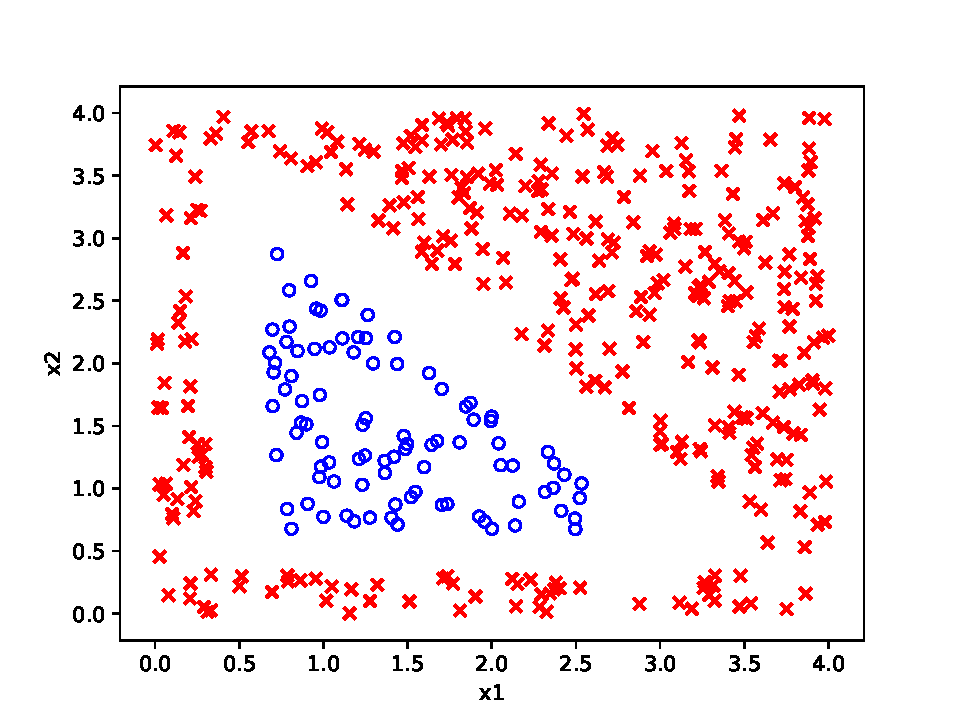
\includegraphics[scale=0.5]{../data/nn_plot.pdf}
		\caption{Plot of dataset $X$.}
		\label{fig:nn_plot}
	\end{figure}

	The examples in class $1$ are marked as as ``$\times$" and examples in class $0$ are marked as ``$\circ$". We want to perform binary classification using a simple neural network with the architecture shown in Figure $\ref{fig:nn_arc}$:
	\begin{figure}[htbp]
		\centering
		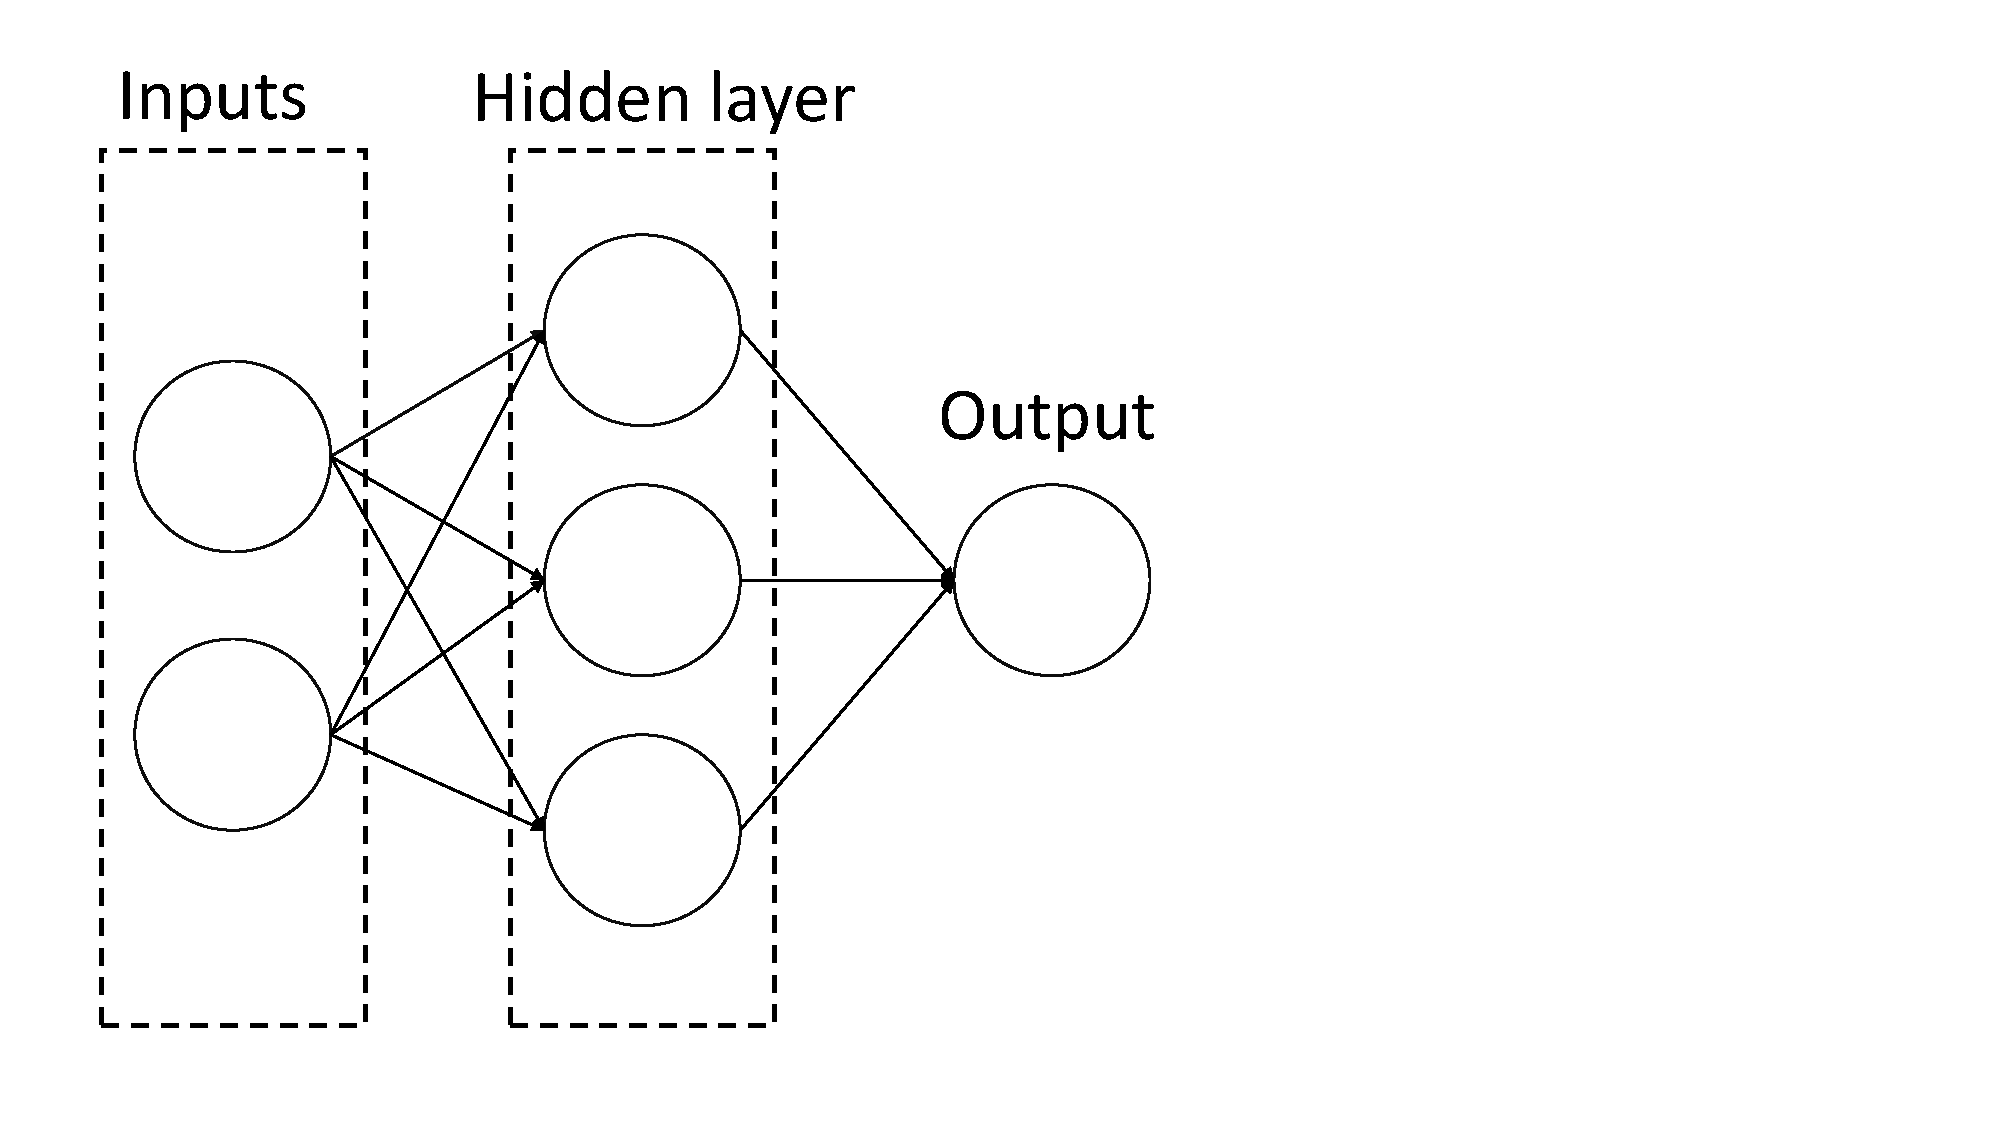
\includegraphics[scale=0.2, trim = 0 0 360 0, clip]{../data/nn_architecture.pdf}
		\caption{Architecture for our simple neural network.}
		 \label{fig:nn_arc}
	\end{figure}

	Denote the two features $x_1$ and $x_2$, the three neurons in the hidden layer $h_1, h_2$, and $h_3$, and the output neuron as $o$. Let the weight from $x_i$ to $h_j$ be $w_{i, j}^{[1]}$ for $i \in \{1, 2\}, j \in \{1, 2, 3\}$, and the weight from $h_j$ to $o$ be $w_{j}^{[2]}$. Finally, denote the intercept weight for $h_j$ as $w_{0, j}^{[1]}$, and the intercept weight for $o$ as $w_{0}^{[2]}$. For the loss function, we'll use average squared loss instead of the usual negative log-likelihood:
  $$l = \frac{1}{m}\sum_{i=1}^{m}(o^{(i)} - y^{(i)})^2,$$
  where $o^{(i)}$ is the result of the output neuron for example $i$.

\begin{enumerate}

  \item \subquestionpoints{5} Suppose we use the sigmoid function as the activation function for $h_1, h_2, h_3$ and $o$.
      What is the gradient descent update to $w_{1, 2}^{[1]}$, assuming we use a learning rate of $\alpha$?
      Your answer should be written in terms of $x^{(i)}$, $o^{(i)}$, $y^{(i)}$, and the weights.\\
      
\ifnum\solutions=1 {
  \begin{answer}
    Let $l^{(i)} = (o^{(i)} - y^{(i)})^2$. Then

    $$
    \frac{\partial l}{\partial w^{[1]}_{1, 2}} = \frac{1}{m}\Sigma_{i=1}^m\frac{\partial l^{(i)}}{\partial w^{[1]}_{1, 2}}
    $$

    Note that $w^{[1]}_{1, 2}$ is only affecting $h_2^{(i)}$. And thus
    $$
    \frac{\partial l^{(i)}}{\partial w^{[1]}_{1,2}} = \frac{\partial l^{(i)}}{\partial o^{(i)}}\frac{\partial o^{(i)}}{\partial h_2^{(i)}}\frac{\partial h_2^{(i)}}{\partial w^{[1]}_{1, 2}}
    $$

    $$
\frac{\partial l^{(i)}}{\partial w^{[1]}_{1,2}} = \frac{\partial l^{(i)}}{\partial o^{(i)}}\frac{\partial o^{(i)}}{\partial h_2^{(i)}}\frac{\partial h_2^{(i)}}{\partial w^{[1]}_{1, 2}}
$$

Since $l^{(i)} = (o^{(i)} - y^{(i)})^2$,
$$
\frac{\partial l^{(i)}}{\partial o^{(i)}} = 2(o^{(i)} - y^{(i)})
$$
Since $o^{(i)} = \sigma(w^{[2]}_0 + w^{[2]}_1 h_1^{(i)} + w_2^{[2]}h_2^{(i)} + w_3^{[3]}h_3^{(i)})$ ,
$$
\frac{\partial o^{(i)}}{\partial h_2^{(i)}} = o^{(i)}(1 - o^{(i)})w_2^{[2]}
$$
And since $h_2^{(i)} = \sigma(w^{[1]}_{0, 2}  + w^{[1]}_{1, 2}x^{(i)}_1+ w^{[1]}_{2, 2}x^{(i)}_2)$,
$$
\frac{\partial h_2^{(i)}}{\partial w^{[1]}_{1, 2}} = h_2^{(i)}(1- h_2^{(i)}) x_1^{(i)}
$$
Combining them we get
$$
\frac{\partial l}{\partial w^{[1]}_{1, 2}} = \sum_{i=1}^m 2(o^{(i)} - y^{(i)})o^{(i)}(1 -  o^{(i)})\sigma(w^{[1]}_{0, 2}  + w^{[1]}_{1, 2}x^{(i)}_1+ w^{[1]}_{2, 2}x^{(i)}_2)(1 - \sigma(w^{[1]}_{0, 2}  + w^{[1]}_{1, 2}x^{(i)}_1+ w^{[1]}_{2, 2}x^{(i)}_2))w_2^{[2]}x_1^{(i)}
$$
        
 \end{answer}

} \fi


  \ifnum\solutions=1 {
  \clearpage
} \fi
\item \subquestionpoints{10} Now, suppose instead of using the sigmoid function for the activation function
      for $h_1, h_2, h_3$ and $o$,
      we instead used the step function $f(x)$, defined as
		\begin{align*}
		f(x) = \begin{cases}
		1, x \ge 0 \\
		0, x < 0
		\end{cases}
		\end{align*}

Is it possible to have a set of weights that allow the neural network to classify this dataset with 100\% accuracy?

If it is possible, please provide a set of weights that enable 100\% accuracy by completing \texttt{optimal\_step\_weights} within \texttt{src/p01\_nn.py} and explain your reasoning for those weights in your PDF.

If it is not possible, please explain your reasoning in your PDF. (There is no need to modify \texttt{optimal\_step\_weights} if it is not possible.)


\textbf{Hint:} There are three sides to a triangle, and there are three neurons in the hidden layer.

\ifnum\solutions=1 {
  \begin{answer}
    It is possible. Three lines can be used to determine the decision boundary. The three lines are
    $$
    \begin{aligned}
        x_1 = 0.5\\
        x_2 = 0.5\\
        x_1 + x_2 = 4
    \end{aligned}
    $$

    If we make 

    $$
    \begin{aligned}
        h_1 = 1 \Leftrightarrow x_1 \le 0.5\\
        h_2 = 1 \Leftrightarrow x_2 \le 0.5\\
        h_3 = 1 \Leftrightarrow x_1 + x_2 \ge 4
    \end{aligned}
    $$

    And 

    $$
        o = 1 \Leftrightarrow h_1 + h_2 + h_3 \ge 1
        $$
    Then $o = 1$ if and only if the points are not in the triangle region. The weights can then be determined using these equations.


 \end{answer}

} \fi

  
  \ifnum\solutions=1 {
  \clearpage
} \fi
\item \subquestionpoints{10} Let the activation functions for $h_1, h_2, h_3$ be the linear function $f(x) = x$ and the activation function for $o$ be the same step function as before.

Is it possible to have a set of weights that allow the neural network to classify this dataset with 100\% accuracy?

If it is possible, please provide a set of weights that enable 100\% accuracy by completing \texttt{optimal\_linear\_weights} within \texttt{src/p01\_nn.py} and explain your reasoning for those weights in your PDF.

If it is not possible, please explain your reasoning in your PDF. (There is no need to modify \texttt{optimal\_linear\_weights} if it is not possible.)


\ifnum\solutions=1 {
  \begin{answer}
    This is impossible. Note in this case
    $$
    \begin{aligned}
        &h = (w^{[1]})^T x\\
        &o = \text{step}((w^{[2]})^T h) = \text{step}((w^{[2]}w^{[1]})^T x)
    \end{aligned}
    $$

    And clearly the decision boundary will be a single line, which cannot separate the two classes.
    
\end{answer}

} \fi


\end{enumerate}
